\documentclass[twoside]{article}
\setlength{\oddsidemargin}{0.25 in}
\setlength{\evensidemargin}{-0.25 in}
\setlength{\topmargin}{-0.6 in}
\setlength{\textwidth}{6.5 in}
\setlength{\textheight}{8.5 in}
\setlength{\headsep}{0.75 in}
\setlength{\parindent}{0 in}
\setlength{\parskip}{0.1 in}
\usepackage{natbib}
\usepackage{amsmath,amsfonts,graphicx}
\usepackage{float}
%
% The following commands set up the lecnum (chap number)
% counter and make various numbering schemes work relative
% to the chap number.
%
\newcounter{lecnum}
\renewcommand{\thepage}{\thelecnum-\arabic{page}}
\renewcommand{\thesection}{\thelecnum.\arabic{section}}
\renewcommand{\theequation}{\thelecnum.\arabic{equation}}
\renewcommand{\thefigure}{\thelecnum.\arabic{figure}}
\renewcommand{\thetable}{\thelecnum.\arabic{table}}

%
% The following macro is used to generate the header.
%
\newcommand{\chap}[4]{
   \pagestyle{myheadings}
   \thispagestyle{plain}
   \newpage
   \setcounter{lecnum}{#1}
   \setcounter{page}{1}
   \noindent
   \begin{center}
   \framebox{
      \vbox{\vspace{2mm}
    \hbox to 6.28in { {\bf SDS 383D: Modeling II
	\hfill Spring 2017} }
       \vspace{4mm}
       \hbox to 6.28in { {\Large \hfill Section #1: #2  \hfill} }
      \vspace{2mm}}
   }
   \end{center}
   \markboth{Section #1: #2}{Section #1: #2}

   
}
%
% Convention for citations is authors' initials followed by the year.
% For example, to cite a paper by Leighton and Maggs you would type
% \cite{LM89}, and to cite a paper by Strassen you would type \cite{S69}.
% (To avoid bibliography problems, for now we redefine the \cite command.)
% Also commands that create a suitable format for the reference list.
%\renewcommand{\cite}[1]{[#1]}
%\def\beginrefs{\begin{list}%
%        {[\arabic{equation}]}{\usecounter{equation}
%         \setlength{\leftmargin}{2.0truecm}\setlength{\labelsep}{0.4truecm}%
%         \setlength{\labelwidth}{1.6truecm}}}
%\def\endrefs{\end{list}}
%\def\bibentry#1{\item[\hbox{[#1]}]}

%Use this command for a figure; it puts a figure in wherever you want it.
%usage: \fig{NUMBER}{SPACE-IN-INCHES}{CAPTION}
\newcommand{\fig}[3]{
			\vspace{#2}
			\begin{center}
			Figure \thelecnum.#1:~#3
			\end{center}
	}
% Use these for theorems, lemmas, proofs, etc.
\newtheorem{theorem}{Theorem}[lecnum]
\newtheorem{lemma}[theorem]{Lemma}
\newtheorem{proposition}[theorem]{Proposition}
\newtheorem{claim}[theorem]{Claim}
\newtheorem{corollary}[theorem]{Corollary}
\newtheorem{definition}[theorem]{Definition}
\newtheorem{exercise}{Exercise}[lecnum]
\newtheorem{example}{Example}[lecnum]
\newenvironment{proof}{{\bf Proof:}}{\hfill\rule{2mm}{2mm}}

% **** IF YOU WANT TO DEFINE ADDITIONAL MACROS FOR YOURSELF, PUT THEM HERE:

\newcommand\E{\mathbb{E}}
\newcommand\Prob{\mathbf{P}}
\newcommand\Q{\mathbf{Q}}
\newcommand\cov{\mbox{cov}}
\begin{document}
\chap{3}{Bayesian GLMs}
\maketitle

\section{Modeling non-Gaussian observations}

So far, we've assumed real-valued observations. In this setting, our likelihood model is a univariate normal, parametrized by a mean $x_i^T\beta$ and some precision that does not directly depend on the value of $x_i$. In general, $x_i^T\beta$ will take values in $\mathbb{R}$


If we don't want to use a Gaussian likelihood, we typically won't be able to parametrize our data using a real-valued parameter. Instead, we must transform it via an appropriate link function. This is, in essence, the generalized linear model.



As a first step into other types of data, let's consider binary valued observations. Here, the natural likelihood model is a Bernoulli random variable; however we cannot directly parametrize this by $x_i^T\beta$. Instead, we must transform $x_i^T\beta$ to lie between $0$ and $1$ via some function $g^{-1}:\mathbb{R}\rightarrow (0,1)$. We can then write a linear model as

$$\begin{aligned}
  y_i|p_i \sim& \mbox{Bernoulli}(p_i)\\
  p_i =& g^{-1}(x_i^T\beta)\\
  \beta|\theta \sim& \pi_\theta(\beta)
\end{aligned}$$


where $\pi_\theta(\beta)$ is our choice of prior on $\beta$. Unfortunately, there is no choice of prior here that makes the model conjugate.

Let's start off with a normal prior on $\beta$. One appropriate function for $g^{-1}$ is the CDF of the normal distribution -- known as the probit function. 
This is equivalent to assuming our data are generated according to

$$\begin{aligned}
  y_i =& \begin{cases} 1 & if z>0 \\ 0 & \mbox{otherwise}\end{cases}\\
  z_i \sim& \mbox{N}(x_i^T\beta, \tau^2)
\end{aligned}$$

If we put a normal-inverse gamma prior on $\beta$ and $\tau$, then we have a \textit{latent} regression model on the $(x_i,z_i)$ pairs, that is idential to what we had before! Conditioned on the $z_i$, we can easily sample values for $\beta$ and $\tau$.

\begin{exercise}
  To complete our Gibbs sampler, we must specify the conditional distribution $p(y_i|x_i,z_i,\beta, \tau)$. Write down the form of this conditional distribution, and write a Gibbs sampler to sample from the posterior distribution. Test it on the dataset \texttt{pima.csv}, which contains diabetes information for women of Pima indian heritage. The dataset is from National Institute of Diabetes and Digestive and Kidney Diseases, full information and explanation of variables is available at \texttt{http://archive.ics.uci.edu/ml/datasets/Pima+Indians+Diabetes}.

\end{exercise}

\textbf{Begin Solution:}
The posterior distribution of the latent variable $z_i$ is
\begin{equation*}
z_i|x_i,y_i,\beta,\omega \sim \Bigg\{\begin{tabular}{c} $N_{\left(0,+\infty \right)}\left(x_i^T\beta,\omega^2 \right)$ if $y_i = 1$\\
$N_{\left(-\infty,0 \right)}\left(x_i^T\beta,\omega^2 \right)$ if $y_i = 0$ \end{tabular}
\end{equation*}
To get samples from the posterior $p\left(\beta|x,y,z,\omega \right)$, choose the following as prior:\\
$a = 0.1,b = 5,k=I_n$
so that $a_n = a + \frac{n}{2}, K_n = X^T X + K, \mu_n = K_n^{-1}\left(X^T z \right), b_n = b + \frac{1}{2}\left(z^T z-mu_n^T K_n \mu_n\right)$
The MCMC samples from the following distribution:\\
$\omega \sim Ga\left(\omega;a_n, b_n \right)$\\
$\beta \sim N\left(\beta;\mu_n,\left( \omega K_n\right)^{-1} \right)$\\
The resulting correct rate is 0.65\\
\textbf{End Solution}

Another choice for $g^{-1}(\theta)$ might be the logit function, $\frac{1}{1+e^{-x^T\beta}}$. In this case, it's less obvious to see how we can construct an auxilliary variable representation (it's not impossible! See \citet{PolScoWin2013}. But for now, we'll assume we haven't come up with something). So, we're stuck with working with the posterior distribution over $\beta$.

\begin{exercise}
  Sadly, the posterior isn't in a ``known'' form. As a starting point, let's find the maximum a posteriori estimator (MAP). The dataset ``titantic.csv'' contains survival data from the Titanic; we're going to look at probability of survival as a function of age. For now, we're going to assume the intercept of our regression is zero -- i.e.\ that $\beta$ is a scalar.  Write a function (that can use a black-box optimizer! No need to reinvent the wheel. It shouldn't be a long function) to estimate the MAP of $\beta$. Note that the MAP corresponds to the frequentist estimator using a ridge regularization penalty.
\end{exercise}

\textbf{Begin Solution:}
To maximize the log likelihood function
\begin{equation*}
\log \left(P\left(\beta \right) \right) = -\frac{1}{2\sigma^2} - \sum_{i} y_i \log \left(1 + \exp\left(-x_i^T \beta \right) \right) -\sum_i \left(1 - y_i \right)\log\left(1 + \exp\left(x_i^T \beta \right) \right) + \lambda\beta^2 - t
\end{equation*}
With initial guess of $\beta = 0.5$, the optimum is found at $\beta^* = -0.011$\\
\textbf{End Solution}

\begin{exercise}
  OK, we don't know how to sample from the posterior, but we can at least look at it. Write a function to calculate the posterior pdf $p(\beta|\mathbf{x},\mathbf{y},\mu,\sigma^2)$, for some reasonable hyperparameter values $\mu$ and $\theta$ (up to a normalizing constant is fine!). Plot over a reasonable range of $\beta$ (your MAP from the last question should give you a hint of a reasonable range).
\end{exercise}

\textbf{Begin Solution:}
The following plot shows the log-likelihood
\begin{figure}[H]
\begin{center}
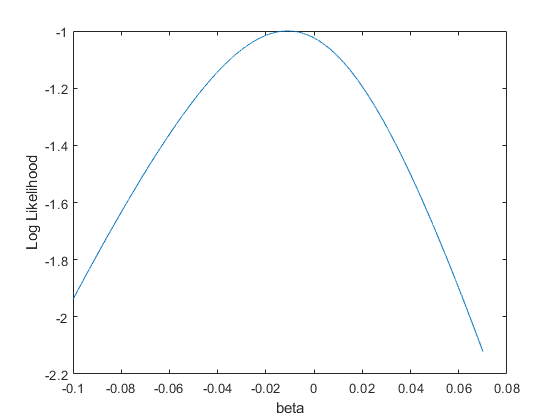
\includegraphics[width=0.5\textwidth]{./figure32.png}
\end{center}
\caption{Exercise 3.3}
\end{figure}
\textbf{End Solution}

The Laplace approximation is a method for approximating a distribution with a Gaussian, by matching the mean and variance at the mode.\footnote{More generally, the Laplace approximation is used to approximate integrands of the form $\int_A e^{Nf(x)} dx$... but for our purposes we will always be working with PDFs.} Let $P^*$ be the (unnormalized) PDF  of a distribution we wish to approximate. We start by taking a Taylor expansion of the log (unnormalized) PDF at the global maximizing value $x^*$

$$\log P^*(x) \approx \log P^*(x^*) - \frac{c}{2}(x-x^*)^2$$

where $c = -\frac{\delta^2}{\delta x^2}\log P^*(x)\Big\rvert_{x=x^*}$.

We approximate $P^*$ with an unnormalized Gaussian, with the same mean and variance as $P^*$:
$$Q^*(x) = P^*(x^*)\exp\left\{-\frac{c}{2}(x-x^*)^2\right\}$$




\begin{exercise}
  Find the mean and precision of a Gaussian that can be used in a Laplace approximation to the posterior distribution over $\beta$.
\end{exercise}

\textbf{Begin Solution:}
\begin{equation*}
\begin{split}
\frac{\partial^2 \log \left(p(\beta|x,y) \right)}{\partial \beta_j^2} \propto -\frac{1}{\sigma^2} - \sum_{i = 1}^n \frac{x_{i_j}^2 \exp\left(x_i^T\beta\right)}{\left(1+\exp\left(x_i^T\beta\right)\right)^2}
\end{split}
\end{equation*}
For a Gaussian distribution $N\left( \mu,\omega\right)$,$\frac{\partial^2 \log (P)}{\partial x^2} = -\omega^2$,$\mu = \beta^*$\\
\textbf{End Solution}

\begin{exercise}
  That's all well and good... but we probably have a non-zero intercept.  We can extend the Laplace approximation to multivariate PDFs. This amounts to estimating the precision matrix of the approximating Gaussian using the negative of the Hessian -- the matrix of second derivatives
$$H_{ij} = \frac{\delta^2}{\delta x_i \delta x_j}\log P^*(x)\Big\rvert_{x=x^*}$$

  Use this to approximate the posterior distribution over $\beta$. Give the form of the approximating distribution, plus 95\% marginal credible intervals for its elements.
\end{exercise}

\textbf{Begin Solution:}
\begin{equation*}
\begin{split}
p(\beta|x,y) &\propto p(y|x,\beta)p(\beta)\\
&\propto N(\beta;0,\sigma^2 I) \prod_{i = 1}^n Bern(y_i;\frac{1}{1+\exp(-x_i^T\beta)})\\
&\propto \exp\left(-\frac{1}{2\sigma^2}\beta^T\beta \right)\prod_{i = 1}^n \left\{ \left[ \frac{1}{1+\exp\left(-x_i^T\beta\right)}\right]^{y_i} \left[1 - \frac{1}{1+\exp \left(-x_i^T\beta \right)} \right]^{1-y_i}\right\}\\
&\propto \exp\left(-\frac{1}{2\sigma^2}\beta^T\beta \right)\prod_{i = 1}^n \left\{\exp\left(x_i^T\beta y_i\right)\cdot \frac{1}{\exp \left(x_i^T \beta\right) + 1} \right\}
\end{split}
\end{equation*}
Take log transformation
\begin{equation*}
\begin{split}
\log\left(p\left(\beta\right) \right) &\propto -\frac{1}{2\sigma^2}\beta^T\beta+\sum_{i = 1}^n\log\left\{\exp\left(x_i^T\beta y_i \right)\cdot \frac{1}{\exp\left(x_i^T\beta \right) + 1} \right\}\\
&= -\frac{1}{2\sigma^2}\beta^T\beta+\sum_{i = 1}^n\left\{x_i^T\beta y_i - \log\left( \exp\left( x_i^T\beta\right) + 1\right) \right\}
\end{split}
\end{equation*}
Compute partial derivatives
\begin{equation*}
\begin{split}
\frac{\partial \log \left(p(\beta|x,y) \right)}{\partial \beta_j} \propto \frac{1}{\sigma^2}\beta_j + \sum_{i = 1}^n \left[x_{i_j}y_i - \frac{x_{i_j}}{1 + \exp\left(-x_i^T\beta \right)} \right]
\end{split}
\end{equation*}

\begin{equation*}
\begin{split}
\frac{\partial^2 \log \left(p(\beta|x,y) \right)}{\partial \beta_j^2} \propto -\frac{1}{\sigma^2} - \sum_{i = 1}^n \frac{x_{i_j}^2 \exp\left(x_i^T\beta\right)}{\left(1+\exp\left(x_i^T\beta\right)\right)^2}
\end{split}
\end{equation*}

\begin{equation*}
\begin{split}
\frac{\partial^2 \log \left(p(\beta|x,y) \right)}{\partial \beta_j \beta_k} \propto -\sum_{i=1}^n\frac{x_{i_j}x_{i_k}\exp\left(x_i^T\beta\right)}{\left(1+\exp\left(x_i^T\beta\right)\right)^2}
\end{split}
\end{equation*}
The values to maximize the posterior distribution is $\beta_{MAP} = [-0.1989,-0.0083]$,plug into the Hessian matrix and the results are
$$
H = \begin{bmatrix}
    -49.67       & -2749 \\
    -2749       & -20200
\end{bmatrix}
$$
The posterior distribution takes the form
$$P(\beta) = \left(\frac{-H}{2\pi} \right)\exp \left\{-\frac{1}{2}\left(\beta - \beta_{MAP} \right)^T\left(-H \right) \left(\beta - \beta_{MAP} \right) \right\} $$\\
%The 95\% CI is $$ for intercept and $$ for age.
\textbf{End Solution}  

  Let's try the same thing with a Poisson likelihood. Here, the obvious transformation is to let $g^{-1}(\theta) = e^{\theta}$, i.e.

$$\begin{aligned}
  y_i|p_i \sim& \mbox{Poisson}(\lambda_i)\\
  \lambda_i =& e^{x_i^T\beta}\\
\end{aligned}$$

  We're going to work with the dataset \texttt{tea\_discipline\_oss.csv}, a dataset gathered by Texas Appleseed, looking at the number of out of school suspensions (ACTIONS) accross schools in Texas. The data is censored for privacy reasons -- data points with fewer than 5 actions are given the code ``-99''. For now, we're going to exclude these data points. 

  \begin{exercise}
    We're going to use a Poisson model on the counts. Ignoring the fact that the data is censored, why is this not quite the right model? \textit{Hint: there are several answers to this -- the most fundamental involve considering the support of the Poisson}.
  \end{exercise}

  
  \begin{exercise}
    Let's assume our only covariate of interest is GRADE\footnote{I have manually replaced Kindergarten and Pre-K with Grades 0 and -1, respectively.} and put a normal prior on $\beta$. Using a Laplace approximation and an appropriately vague prior, find  95\% marginal credible intervals for the entries of $\beta$. You'll probably want to use an intercept.
  \end{exercise}

  \begin{exercise}[Optional]
    Repeat the analysis using a set of variables that interest you.
  \end{exercise}


      Even though we don't have conjugacy, we can still use MCMC methods -- we just can't use our old friend the Gibbs sampler. Since this isn't an MCMC course, let's use STAN, a probabilistic programming language available for R, python and Matlab. I'm going to assume herein that we're using RStan, and give appropriate scripts; it should be fairly straightforward to use if you're an R novice, or if you want to use a different language, there are hints on translating to PyStan at \texttt{http://pystan.readthedocs.io/en/latest/differences\_pystan\_rstan.html} and info on MatlabStan (which seems much less popular) at \texttt{http://mc-stan.org/users/interfaces/matlab-stan}.
  \begin{exercise}
    Download the sample STAN script \texttt{poisson.stan} and corresponding R script \texttt{run\_poisson\_stan.R}. The R script should run the  regression vs GRADE from earlier (feel free to change the prior parameters). Run it and see how the results differ from the Laplace approximation. Modify the scripy to include more variables, and present your results.
  \end{exercise}

  
  \begin{exercise}
    Consider ways you might improve your regression (still, using the censored data) - while staying in the GLM framework.  Ideas might include hierarchical error modeling (as we looked at in the last set of exercises), interaction terms... or something else! Looking at the data may give you inspiration. Implement this in STAN.
  \end{exercise}
    
  
  \begin{exercise}
    We are throwing away a lot of information by not using the censored data. Come up with a strategy, and write down how you would alter your model/sampler. Bonus points for actually implementing it in STAN (hint: look up the section on censored data in the STAN manual).
  \end{exercise}

  \bibliographystyle{apalike}
  \bibliography{course}

\end{document}
